% Beamer Presentation Template
% Author: Primal Pappachan
% Last Updated: 4 - 10 - 2011
% 

\documentclass[compress,red]{beamer} %

\usetheme{Warsaw}
% other themes: AnnArbor, Antibes, Bergen, Berkeley, Berlin, Boadilla, boxes, CambridgeUS, Copenhagen, Darmstadt, default, Dresden, Frankfurt, Goettingen,
% Hannover, Ilmenau, JuanLesPins, Luebeck, Madrid, Maloe, Marburg, Montpellier, PaloAlto, Pittsburg, Rochester, Singapore, Szeged, classic

\usepackage[latin1]{inputenc}
\usefonttheme{professionalfonts}
\usepackage{times}
\usepackage{tikz}
\usepackage{amsmath}
\usepackage{verbatim}
\usepackage{url}
\usepackage{graphics}
\usepackage{subfigure}

%\usecolortheme{default}
% color themes: albatross, beaver, beetle, crane, default, dolphin, dov, fly, lily, orchid, rose, seagull, seahorse, sidebartab, structure, whale, wolverine

\useoutertheme[subsection=false]{smoothbars}

\usefonttheme[onlysmall]{structurebold}

% font themes: default, professionalfonts, serif, structurebold, structureitalicserif, structuresmallcapsserif

\setbeamerfont{title}{shape=\itshape,family=\rmfamily}
%\setbeamercolor{title}{fg=black!80!black,bg=red!90!white}

\logo{} %\logo{\includegraphics[height=0.5cm]{logo.pdf}}
%% Use \insertlogo to insert the logo at place

\title{FOSSEE}
\subtitle{Free and Open source Software for Science and Engineering
Education}
\author[]{www.fossee.in}  %\author[Euclid]{Euclid of Alexandria
\institute{IIT Bombay}
\date[]{} %\date[ISPN ’80]{27th International Symposium of Prime Numbers}


\begin{document}

\begin{frame}
	 \titlepage
\end{frame}

\begin{frame}
\section*{Outline}
\tableofcontents
\end{frame}


\section{FOSS}
\begin{frame}
\frametitle{FOSS}
\begin{definition}
\alert{FOSS} stands for Free and Open Source Software in Science and Engineering
\end{definition}
\end{frame}

\subsection{What can users do?}
\begin{frame}
\frametitle{What users can do?}
\begin{block}{Benefits}
\begin{itemize}
\item See and modify the source code \pause
\item Redistribute and improve the source code \pause
\item Use the software for any purpose 
\end{itemize}
\end{block}
\end{frame}

\subsection{For whom?}
\begin{frame}
\frametitle{FOSS is advantageous for}
\begin{enumerate}
\item Private Industries \pause
\item Entrepreneurs \pause
\item Defence Establishments \pause
\item Research Organisations \pause
\item Academic Institutions\pause
\item Individual User \pause
\end{enumerate}
\begin{block}{FOSS for everyone} \pause
FOSS is for anyone who uses Computer to get things done quickly and efficiently. 
\end{block}
\end{frame}


\section{FOSSEE}

\subsection{FOSSEE at IITB}
\begin{frame}
\frametitle{FOSSEE}
\begin{block}{Stands for}
Free and Open source Software for Science and Engineering
Education \pause
\end{block}
\begin{center}
\vspace*{0.25cm}

\includegraphics[scale=2]{fossee.png} \pause
\end{center}
\vspace*{0.25cm}
\begin{overlayarea}{\textwidth}{5cm}
\only<3>{Based at IIT Bombay}
\only<4>{Funded by MHRD}
\only<5>{Part of National Mission on Education through ICT}
\end{overlayarea}
\end{frame}

\subsection{Goals}
\begin{frame}
\frametitle{Goals}
\begin{itemize}
\item Promote \alert{FOSS} packages to minimize use of commercial tools in science and engineering education \pause
\item Documenation for supported \alert{FOSS} packages \pause
\item Awareness among students and teachers about supported \alert{FOSS} packages   
\end{itemize}
\end{frame}

\subsection{People}
\begin{frame}
\frametitle{People}
\begin{itemize}
\item Prof. Prabhu Ramachandran \\ 
{\footnotesize Aerospace Engineering} \pause
\item Prof. Madhu Belur \\
{\footnotesize Electrical Engineering} \pause
\item Prof. Mani Bhushan \\
{\footnotesize Chemical Engineering}  \pause
\item Prof. Kannan Moudgalya \\
{\footnotesize Chemical Engineering}  
\end{itemize}
\end{frame}

\subsection{Block Diagram}
\begin{frame}
\frametitle{FOSSEE Projects}
\begin{center}
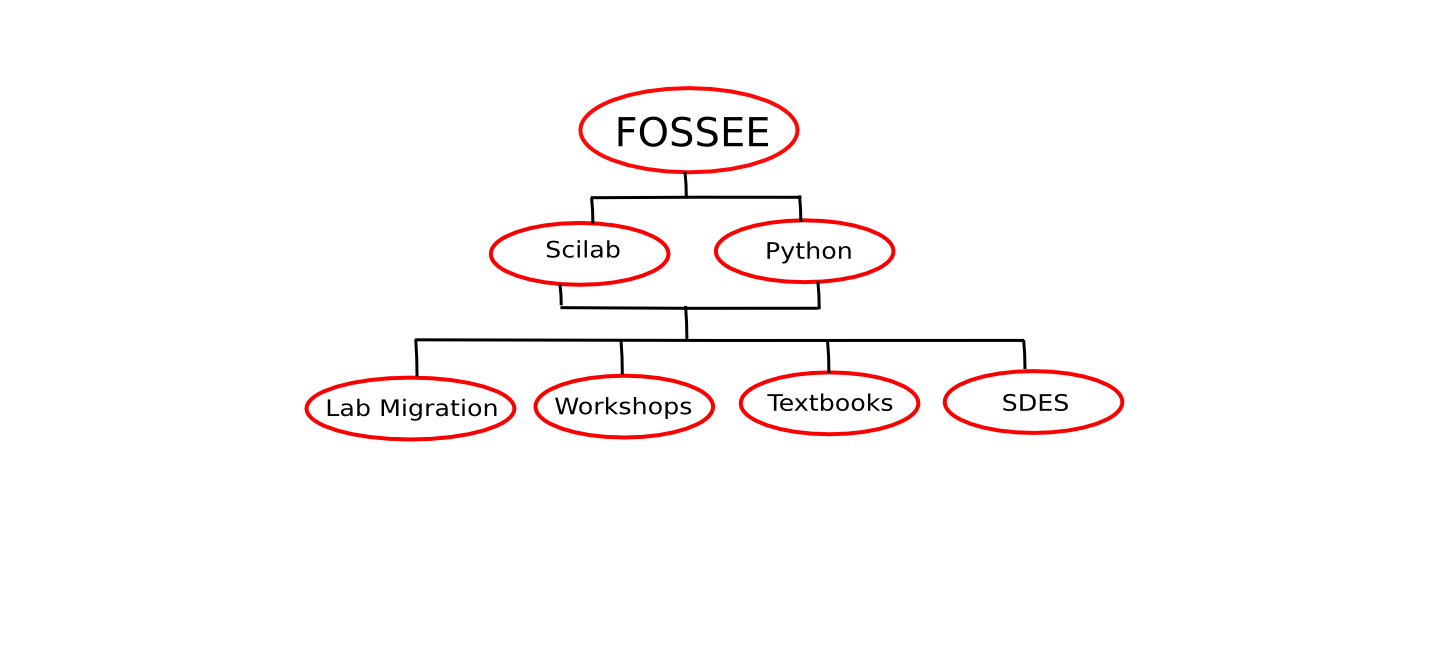
\includegraphics[scale=0.3]{blockdiagram.png}
\end{center}
\end{frame}

\subsection{At IITB}
\begin{frame}
\frametitle{FOSSEE focus at IITB}
\begin{itemize}
\item Python family \pause
   \begin{itemize}
   \item Python
   \item NumPy
   \item SciPy
   \item Sage \pause
   \end{itemize}
\item Scilab family \pause
   \begin{itemize}
   \item Scilab
   \item Xcos \pause
   \end{itemize}
\item Other FOSS actively pursued/used \pause
   \begin{itemize}
   \item GNURadio
   \item KiCA
   \item OpenFOAM
   \item Ngspice
   \item \LaTeX % \Latex \Latex \pause
   \end{itemize}
\end{itemize}
\end{frame}

\section{Activities}

\subsection{Thrust Areas}
\begin{frame}
\frametitle{Thrust Activities}
\begin{itemize}
\item SDES Course \pause
\item Workshops  \pause
\item Textbook Companion Project  \pause
\item Spoken Tutorials \pause
\end{itemize}
\end{frame}

\subsection{SDES}
\begin{frame}
\frametitle{SDES}
\begin{block}{SDES}
Software Development Techniques for Scientists and Engineers
\end{block}
\begin{itemize}
\item Equips a student with various FOSS tools for curricular purposes \pause
\item For students of BE/BTech and ME/MTech programmes \pause
\item Currently in curriculum : IIT Bombay, Varanasi and Chennai \pause
\item Coordinators' workshop was held in September 2011 \pause
\end{itemize}
\end{frame}

\begin{frame}
\frametitle{Teacher's training Workshop}
\begin{itemize}
\item Introduce the faculty of various engineering colleges to advantages of FOSS. \pause
\item Motivate them to include SDES course in their curriculum. \pause
\item Conducted in 2 parts
\begin{enumerate}
\item At IIT \pause
\item Through AVIEW \pause
\end{enumerate}
\end{itemize}

\begin{block}{Large Picture}
From all over India, over {\Large 1000} Teacher's will be trained.
\end{block}
\end{frame}

\subsection{Workshops}
\begin{frame}
\frametitle{Workshops all over India}
\begin{center}
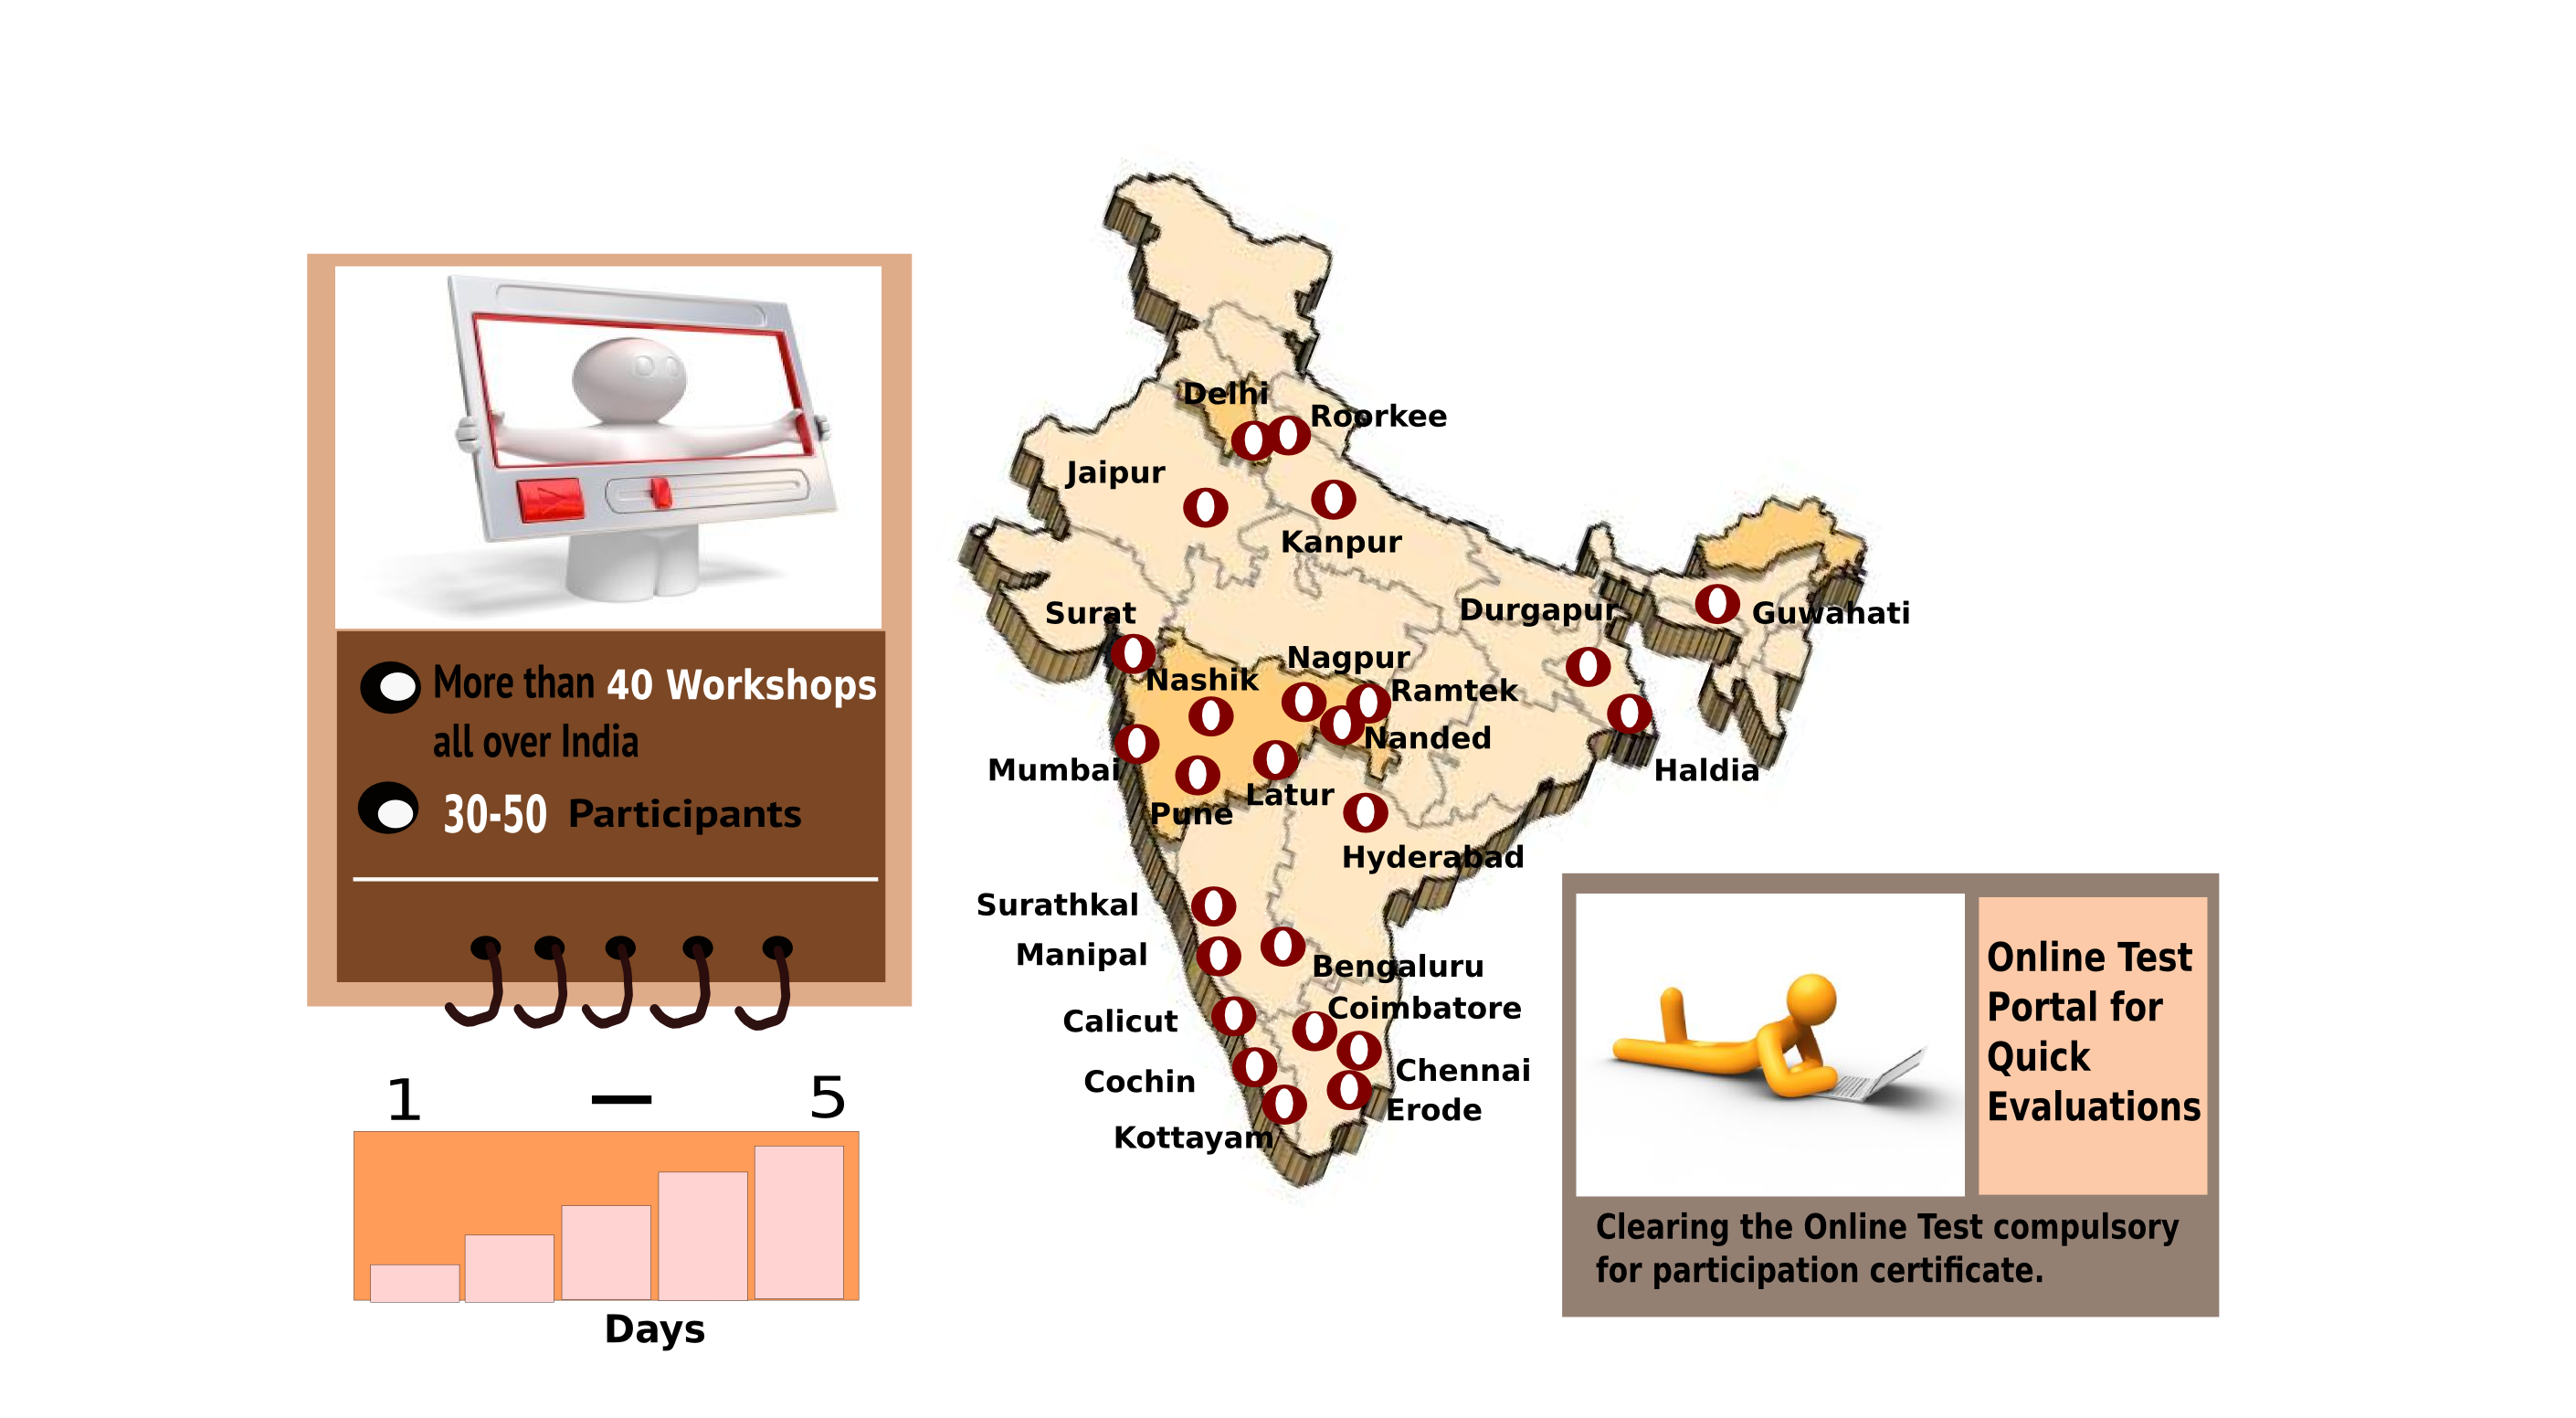
\includegraphics[scale=.15]{workshop.png}
\end{center}
\end{frame}

\subsection{Spoken Tutorials}
\begin{frame}
\frametitle{Spoken Tutorials}
\begin{columns}
\column{.5\textwidth}
\begin{block}{On}
\begin{itemize}
\item Scilab \pause
\item Python - Basic and Advanced \pause
\item \LaTeX \pause
\item Version Control \pause
\item Linux utilities \pause
\end{itemize}
\end{block}
\column{.5\textwidth}
\begin{block}{For}
\begin{itemize}
\item Self Learning and Teaching purposes \pause
\item Over \alert{50} tutorials already completed \pause
\end{itemize}
\end{block}
\pause
\end{columns}
\begin{block}{Website}
http://www.spoken-tutorial.org
\end{block}
\end{frame}


\subsection{TextBook Companion Project}

\begin{frame}
\frametitle{TextBook Companion Project}
\begin{block}{Goal}
Create a repository of reference material in the form of solved problems for Scientific Computing with Open Source tools.
\end{block}
\end{frame}

\begin{frame}
\frametitle{How it works?}
\begin{figure}
\centering
\mbox{
\subfigure{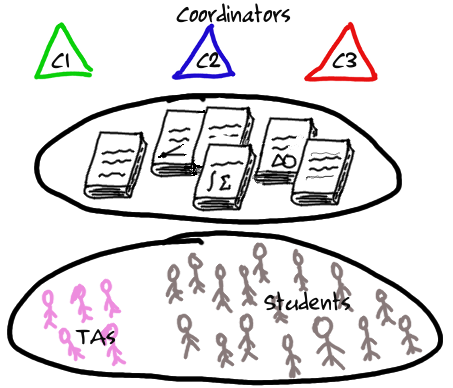
\includegraphics[width=1.5in,height=1.5in]{1.png}} \pause
\subfigure{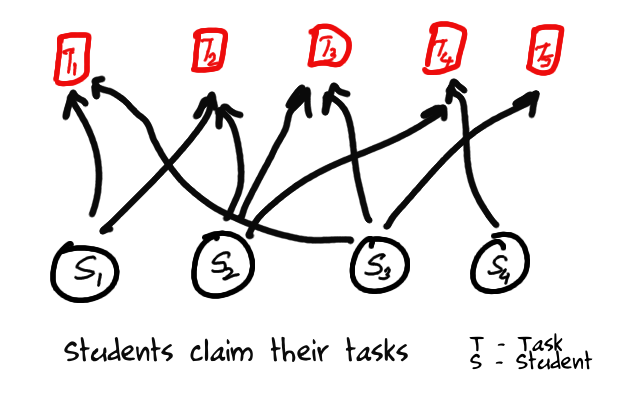
\includegraphics[width=1.5in,height=1.5in]{2.png}} \pause
\subfigure{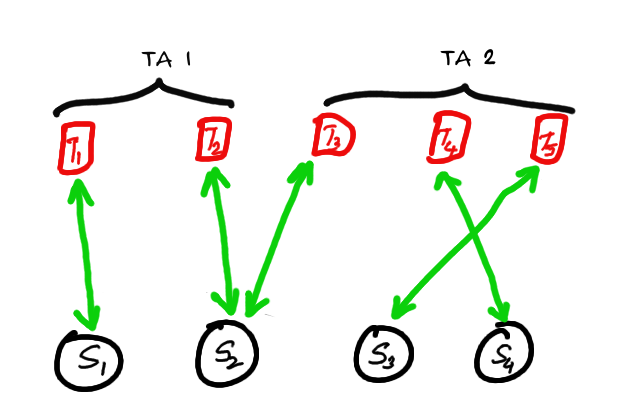
\includegraphics[width=1.5in,height=1.5in]{3.png}}} 
\end{figure}
\end{frame}

\begin{frame}
\frametitle{Statistics}
\begin{center}
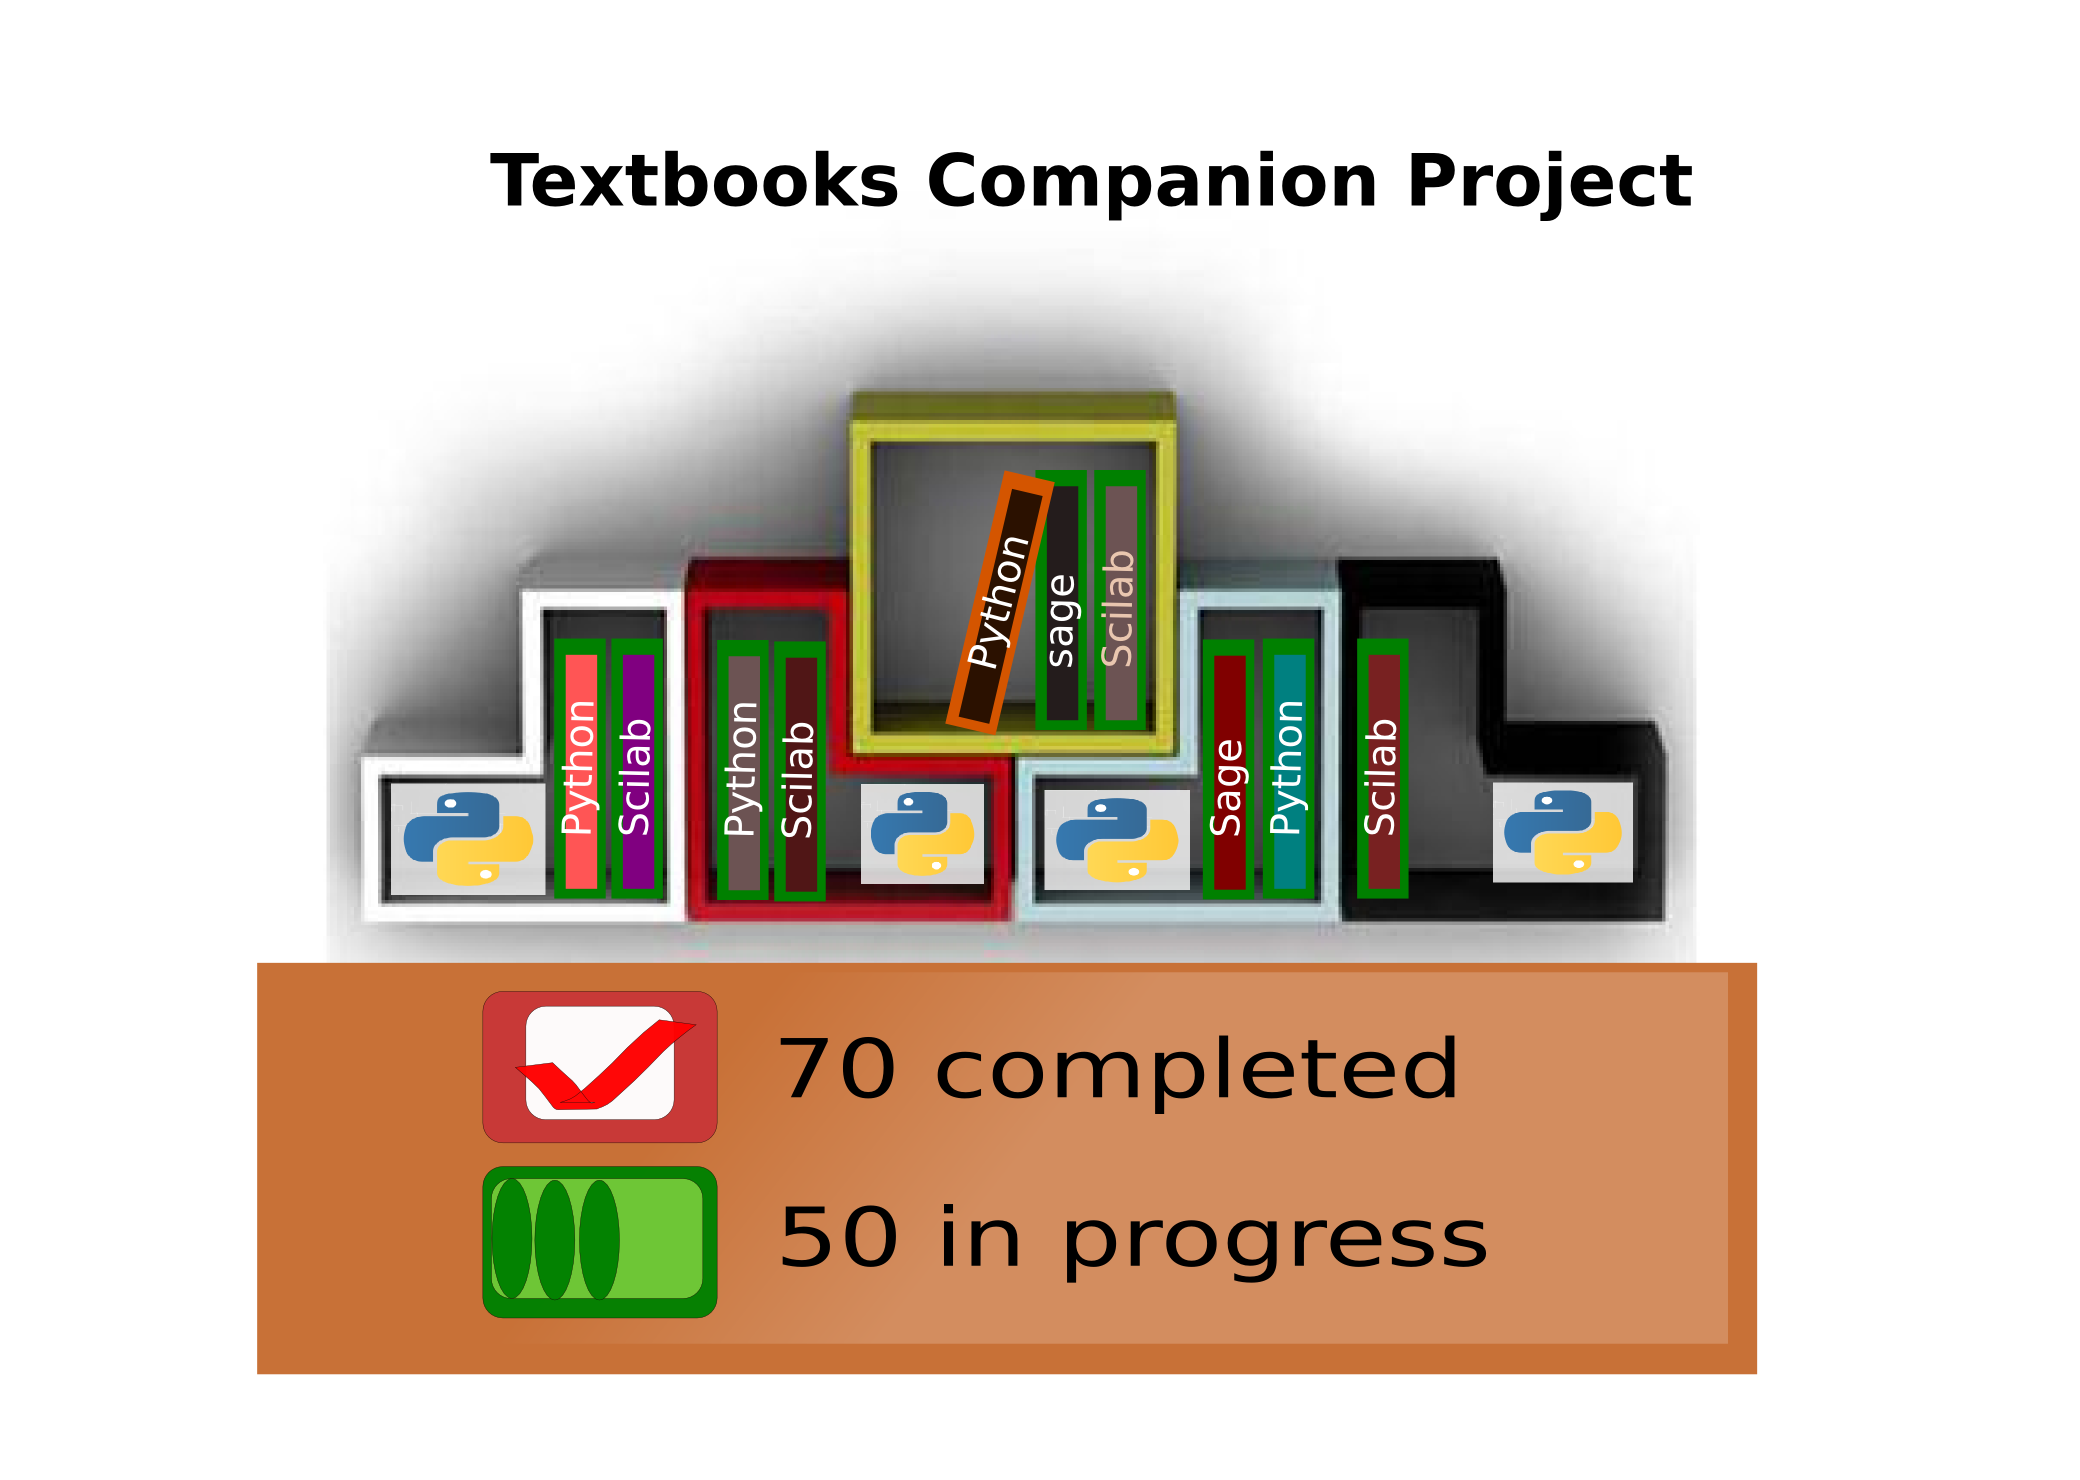
\includegraphics[scale=.15]{textbook.png}
\end{center}
\end{frame}

\subsection{Achievements}
\begin{frame}
\frametitle{Achievements}
\small \bf
{\bf so far (August 2011), till March 2012, till July 2012}
% {\bf Deliverables} % please give milestones with timelines linking with payments
\begin{center}
\begin{table}[h]
\begin{tabular}{|l|c|c|c|}
\hline 
Item & Aug '11 & Mar '12 & Jul '12 \tabularnewline
& (achieved) & (expected) & (proposed) \tabularnewline
\hline
\hline 
Workshops\footnote{\bf These are 1 to 5 days workshop targetted towards
\alert{teachers}, and \alert{evaluated online} before issuing a participation
certificate}  & 40 &  55 & 70\tabularnewline
\hline 
Conferences & 5 & 6 & 7 \tabularnewline
\hline 
Textbook Companions & 51 & 100 & 200 \tabularnewline
\hline 
Spoken Tutorials & 45 & 60 & 70 \tabularnewline
\hline 
Course conversion & 5 & 5 & 5\tabularnewline
\hline
Lab Migration & 4 & 10 & 20 \tabularnewline
\hline
\end{tabular}
\end{table}
\end{center}
\end{frame}

\section*{}
\begin{frame}
    \begin{center}
        \huge
        Thank you\\ \pause
    \end{center}
\end{frame}

\end{document} 